%!TEX root = ./main.tex

\section{Introduction}

%% short online algorithm
Online computation (coined by \cite{BorodinEl-Yaniv05:Online-computation}) is a well-established field in theoretical computer science. Online computational models consider inputs as request sequences, where each request arrives individually over time. After observing the current request, the problem-solving algorithm must perform an irrevocable action without additional information about the future. The performance of an online algorithm is typically measured by the competitive ratio metric, which is the worst ratio between the objective value obtained by the algorithm and that of the optimal solution. Intuitively, the competitive ratio measures the price of not knowing future requests. Our goal is to design performant algorithms within this metric.

%% machine learning as a way to go beyond the worst case
The traditional worst-case analysis is an indispensable framework in algorithm design and is central in the development of algorithms. Nevertheless, it can lead practical users to several pitfalls. Summarizing an algorithm's performance by a pathological worst-case can overestimate its performance on average. Many algorithms that perform well in practice admit mediocre theoretical guarantees, while others which are well-established in theory behave poorly, even on simple instances. Consequently, it is crucial to research theories that can better explain the performance of algorithms and advise algorithm design choices (\cite{Roughgarden19:Beyond-worst-case,Roughgarden20:Beyond-the-Worst-Case}).

%% recent trends
Much of the research focused on going beyond the worst-case paradigm is motivated by the spectacular advances of machine learning (ML). Specifically, ML methods can detect patterns among the arriving input requests and provide valuable insights for the online algorithms regarding future requests. \cite{LykourisVassilvtiskii18:Competitive-caching} introduced a general framework to integrate ML predictions into classical algorithm designs to surpass the worst-case performance limit.
Shortly after, \cite{MitzenmacherVassilvitskii20:Beyond-the-Worst-Case}
followed this line of research and studied online algorithms with predictions. As a result of these papers, many practically relevant online problems were revisited to enhance existing classical algorithms with ML predictions. For example, scheduling (\cite{LattanziLavastida20:Online-scheduling,Mitzenmacher20:Scheduling-with}), caching (\cite{LykourisVassilvtiskii18:Competitive-caching,Rohatgi20:Near-optimal-bounds,AntoniadisCoester20:Online-metric}), and ski rental (\cite{GollapudiPanigrahi19:Online-algorithms,KumarPurohit18:Improving-online}).

Even though predictions provide a glimpse of the future, there is no mathematical guarantee for their accuracy. Adjusting the algorithm's trust in the predictions is a significant challenge since online algorithms must make irrevocable decisions at each time step. Ideally, if the predictions are accurate, the algorithm should perform well compared to the offline setting. In contrast, if the predictions are misleading, the algorithm should maintain a competitive solution, similar to the online setting where no predictive information is available. In other words, online algorithms with predictions are expected to bring the best of both worlds: mathematical performance guarantees of classical algorithms and good future prediction capabilities of machine learning methods.

%% unified methods/primal-dual
To overcome the issue of unknown prediction accuracy, the authors of the works we cited previously exploited specific structures within the studied problems. \cite{BamasMaggiori20:The-Primal-Dual-method} presented a primal-dual method based technique to unify these different ad-hoc approaches and design online algorithms with predictions for various online problems. The primal-dual method is an elegant and powerful algorithm design technique (introduced by \cite{WilliamsonShmoys11:The-design-of-approximation}), especially for online algorithms (see \cite{BuchbinderNaor09:Online-primal-dual}). The work of \cite{BamasMaggiori20:The-Primal-Dual-method} focuses on problems with linear objectives and covering constraints. Until now, it remained an open question to design online algorithms with predictions for \emph{non-linear} covering problems. Non-linear objectives appear naturally in diverse application domains, such as energy and congestion management, or online mixed packing and covering problems. Therefore, answering this open question has high theoretical interest and vital practical motivations. Our paper presents a framework to create online primal-dual algorithms with predictions for covering problems with non-linear objectives.


\subsection{Model}  	\label{sec:model}

Building upon the work of \cite{BamasMaggiori20:The-Primal-Dual-method} (which has several definitions rooted in \cite{LykourisVassilvtiskii18:Competitive-caching,KumarPurohit18:Improving-online}), our model includes a prediction oracle $\mathcal{P}$ and a parameter $\eta \in (0,1]$ which characterizes the confidence in the predictions. Small $\eta$ values represent low doubt, meaning that the prediction accuracy is high, while large $\eta$ values show high doubt, signalling that the predictions should be discarded. Given an online problem, upon the arrival of the current request, the online algorithm solving the problem must make an irrevocable decision regarding the request while satisfying the problem's constraints. In our setting, the decision-making is influenced by the prediction of the oracle $\mathcal{P}$, the confidence parameter $\eta$, the current solution, and the history of released requests. Intuitively, the oracle's predictions provide information about the unknown future. For example, it can predict the optimal machine for the current task during scheduling. To characterize the performance of an online algorithm with predictions, we use the notion of consistency and robustness. An algorithm $\mathcal{A}$ (for a minimization problem) is $C(\eta)$-\emph{consistent} and $R(\eta)$-\emph{robust} if for every instance $I$,
%
\begin{align*}
    %\mathcal{A}(I) 	\geq 	\max\{C(\eta) \cdot \mathcal{P}(I), R(\eta) \cdot \mathcal{O}(I) \}  &\qquad	\text{(maximization problem)}, \\
    \mathcal{A}(I) 	\leq 	\min\{C(\eta) \cdot \mathcal{P}(I), R(\eta) \cdot \mathcal{O}(I) \}  %&\qquad	\text{(minimization problem)},
\end{align*}
%
where $\mathcal{A}(I), \mathcal{P}(I), \mathcal{O}(I)$ are respectively the objective values on instance $I$ of algorithm $\mathcal{A}$, the prediction oracle $\mathcal{P}$ and the optimal offline solution $\mathcal{O}$. Following the convention, when the prediction oracle $\mathcal{P}$ provides an infeasible solution, $\mathcal{P}(I)$ is set to $-\infty$ and $+\infty$ for maximization and minimization problems, respectively. Ideally, when $\eta$ approaches $0$ (high confidence in the prediction), $C(\eta)$ should tend to 1. Meanwhile, when $\eta$ approaches $1$ (high doubt in the prediction), $R(\eta)$ should tend towards the best competitive ratio in the classic online setting.

Similarly to the work of \cite{BamasMaggiori20:The-Primal-Dual-method}, our algorithm $\mathcal{A}$ combines the predictions of oracle $\mathcal{P}$ with the primal-dual method. This method formulates the studied problem as a mathematical program called the primal and its corresponding dual. Considering an online problem, at the arrival of a new request, a primal-dual method based online algorithm updates its fractional solutions to both the primal and dual programs to maintain feasibility (satisfy the constraints of the mathematical programs). The competitive ratio of such an algorithm is established by showing that every time the algorithm updates the primal and dual solutions, the increase of the primal objective value can be bounded by that of the dual up to some desired factor.

Our presented model contains two components by design. One relates to the prediction oracle, and the other to the classical primal-dual method. This duality is also present during the performance evaluation since our algorithms must achieve both good consistency and robustness. Given two separate algorithms, where one blindly follows the predictions while the other makes decisions solely based on the primal-dual method, a natural question is whether a simple linear combination of the two algorithms performs well. If we target a consistency of at least $O(1/(1-\eta))$, using a linear combination of the two algorithms, the robustness must be $\Omega(1/\eta)$. However, the ultimate goal is to achieve robustness in the order of $\text{poly}(\log(1/\eta))$ (exponentially smaller than $\Omega(1/\eta)$) while maintaining $O(1/(1-\eta))$ consistency. Therefore, a simple linear combination of the two components is insufficient to reach the desired performance guarantees.

Our paper presents a framework for non-linear online covering problems with an intricate combination of the classic primal-dual method and a prediction oracle. Algorithms created with our framework construct fractional solutions, which is the primary step in primal-dual method based algorithms. Even though many real-life problems require integer solutions, online rounding schemes already exist for most of them.   We provide references to such rounding schemes at the analysis of our studied problems.


\subsection{Contribution}  \label{sec:intro-covering}

Inspired by the approach of \cite{BamasMaggiori20:The-Primal-Dual-method}, our model (detailed previously) combines an oracle's predictions with the primal-dual method in a way that the oracle's predictions influence the updates of the primal and dual variables. The construction of our algorithm follows the multiplicative weight update method based on the gradient of the multilinear extension of the problem's objective function (\cite{Thang20:Online-Primal-Dual}, see section \ref{sec-prelim}~Preliminaries). This technique generalizes the multiplicative weight update introduced in \cite{BuchbinderNaor09:The-Design-of-Competitive,AzarBuchbinder16:Online-Algorithms}. Using the local-smoothness notion of the multilinear extension, we can prove the feasibility of the primal and dual solutions (even when the prediction is infeasible). Afterwards, the algorithm's performance is established using the local-smoothness and confidence parameters.


\begin{restatable}{theorem}{Covering}
\label{thm:covering}
(Informal definition.) Given a non-linear online covering problem, let $F$ be the multilinear extension (see section \ref{sec-prelim}~Preliminaries) of the problem's objective function. Assuming ($\lambda$,$\mu$)-local-smoothness properties on $F$, for every confidence parameter $\eta$ of the prediction oracle, where $\eta \in (0,1]$, there exists an $O\bigl( \frac{1}{1 - \eta} \bigr)$-consistent and
$O\bigl( \frac{\lambda}{1 - \mu}  \cdot \ln \left(\frac{d}{\eta}\right) \bigr)$-robust algorithm for the non-linear online fractional covering problem, where $d$ is the maximum raw sparsity of the problem's constraints (maximum number of non-zero coefficients in a constraint).
\end{restatable}

%\begin{figure}
%    \centering
%    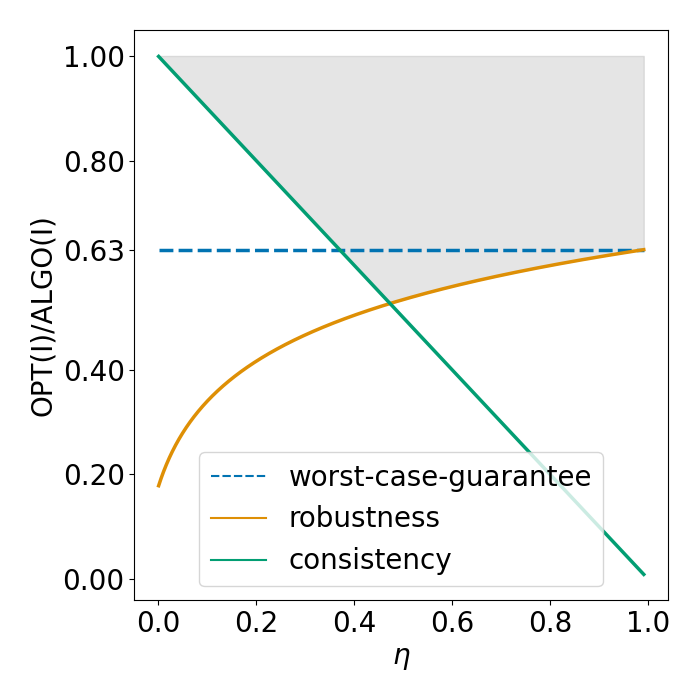
\includegraphics[width=0.5\linewidth]{../../01_covering_multiple_experts/paper/Img/consistency_robustness.png}
%    \caption{Robustness-Consistency}
%    \label{fig:worst-case}
%\end{figure}
%
%\subsubsection{Illustration} Since Theroem~\ref{thm:covering} relies on several parameters, it may be challenging to appreciate its importance. As an example, when the objective function of our problem is a polynomial of degree~$k$, the competitive ratio of state-of-the-art online algorithms \emph{without} predictions is in $O(k^k log(d))$. Meanwhile, the consistency of our framework is $O(1 / (1-\eta))$ and the robustness is $O(k^k log(d/\eta))$. Figure~\ref{fig:worst-case} displays the case when $k = 1$, $d=5$, and the prediction oracle is perfect (the predictions correspond to the ground truth). The competitive ratio of our framework is the shaded area above the consistency and robustness curves. By choosing a small enough $\eta$ value, it is possible to surpass the previous worst-case bound of the state-of-the-art algorithm. If the polynomial degree of the objective function increases, the robustness curve and the state-of-the-art line will decrease drastically (multiplication with $1/k^k$). Similarly, if the prediction oracle is imperfect, the consistency line will tend downwards. However, if the oracle produces a solution at most up to a factor of $k^k$ times the optimal one, it is still possible to surpass previous worst-case guarantees.


We show the applicability of our framework through several problems such as online norm minimization, online mixed packing and covering,
energy minimization, and submodular minimization (\cref{sec:app}).
As a by-product, our work implies the \emph{optimal} competitive ratio of $O\bigl( k \cdot \log (d)\bigr)$
for the standard (without predictions) online problem of minimizing $\|C \vect{x}\|_{k}$ under covering constraints, answering an open question in \cite{NagarajanShen17:Online-Covering} (\cref{appix-norm}). Subsequently, it also provides the \emph{optimal} competitive ratio for the online mixed packing and covering problem (Section \ref{appix-mixed}).

%\subsection{Applications}
%We show the applicability of our framework through the following problems.
%
%\subsection{Online Norm minimization}
%
%Norm functions appear naturally in optimization problems when we want to approximate non-smooth functions (for example the maximum) with smooth ones. Good examples are congestion management and load balancing problems, or machine learning techniques where the norm function is a regularizer. Our proposed algorithm achieves an $O(\frac{1}{1 - \eta})$-consistent and $O\bigl( k \cdot \log (d/\eta)\bigr)$-robust fractional solution for the problem of minimizing $\|C \vect{x}\|_{k}$ under covering constraints. We highlight that in the standard online setting where there are no predictions, the algorithm is  $O\bigl( k \cdot \log (d)\bigr)$-competitive, which is asymptotically \emph{optimal} (see the lower bound established in \cite{AzarCohen14:Online-Covering}). Furthermore, this result answers an open question from \cite{NagarajanShen17:Online-Covering}.
%
%\subsection{Online mixed packing and covering}
%
%The online mixed packing and covering problem is a good example for the importance of the norm function. Given a set of offline packing constraints ($C \vect{x} \leq \one$) and a set of online covering constraints ($B \vect{x} \geq \one$), our goal is to gradually increase the decision variable $\vect{x}$ such that the covering constraints are satisfied, while the packing constraints are violated as little as possible. Formally, $B \vect{x} \geq \one$ holds, while the factor~$\xi$ by which $C \vect{x} \leq \xi \cdot \one$ is as small as possible. We can reformulate this problem as $\min \| C \vect{x}\|_{\infty}$ subject to online constraints $B \vect{x} \geq \one$. The $\ell_{\log m}$-norm is a constant approximation for the $\ell_{\infty}$-norm, so our proposed algorithm is $O(\frac{1}{1 - \eta})$-consistent and $O\bigl( \log k \cdot \log (d/\eta)\bigr)$-robust. We highlight that in the standard online setting where there are no predictions, the algorithm is $O\bigl( \log m \cdot \log d \bigr)$-competitive, which is \emph{optimal} up to a constant factor (see the lower bound in \cite{AzarBhaskar13:Online-mixed}).
%
%\subsubsection{Energy Minimization in Scheduling}
%Reducing carbon emissions is a global effort in which energy-efficient algorithms play an essential role. For example, \cite{Albers10:Energy-efficient-algorithms} and \cite{GuCaiZengZhangJinDai:2019} studied energy-efficient algorithms for scheduling. Contrary to performance-oriented scheduling, our goal is to design an assignment policy of jobs to $m$ available machines, which can minimize the total energy consumption of the execution. Energy-related objective functions are typically polynomials of degree $k > 1$. Using our proposed framework, we can derive an $O(\frac{1}{1 - \eta})$-consistent and $O\bigl(k^{k} \log^{k} \frac{m}{\eta}\bigr)$-robust algorithm with fractional solutions for this energy minimization problem.
%
%\subsubsection{Submodular Minimization}
%Submodular minimization is a widespread subject in optimization and machine learning (\cite{IwataFleischer01:A-combinatorial-strongly,Bachothers13:Learning-with,Bach16:Submodular-functions:,BalkanskiSinger:2020}). We present a
%$O(\frac{1}{1 - \eta})$-consistent and $O\bigl( \frac{\log (d/\eta)}{1 - \kappa_{f}} \bigr)$-robust algorithm
%for minimizing a submodular function under covering constraints where $\kappa_{f}$ is the curvature
%(defined in \cref{sec:sub-min}) of the submodular function.

\subsection{Experiments}
The experiments focus on a high-impact congestion management problem: network and transportation routing. The input is a directed graph $G(A,V)$ and a set of requests $R = \{(s_{i}, t_{i}) : s_{i}, t_{i} \in V\}$ that represents demands (connecting $s_{i}$ to $t_{i}$ through a path). Each arc $(u, v) \in A$ is associated with a cost function $f_{(u,v)}: \mathbb{R}^{+} \rightarrow \mathbb{R}^{+}$ that depends on the number of requests using the arc. The goal is to design a routing that minimizes the total cost while requests arrive online. We enable predictions by building an oracle using the observed data. The oracle provides traffic forecasts, vital information to improve the routing. The experiments show that in some cases our algorithm outperforms both the best theoretical algorithm and the prediction in practical settings. The details of the experiments are available in \cref{sec:exp}.


\subsection{Related work}
% Primal-Dual
The primal-dual method is a powerful tool in online optimization. \cite{BuchbinderNaor09:The-Design-of-Competitive} introduced a primal-dual framework for linear programs with packing and covering constraints. Their method unifies several previous potential-function-based analyses and gives a principled approach to the design and analysis of algorithms for problems with linear relaxations. \cite{AzarBuchbinder16:Online-Algorithms} provided a framework for covering and packing problems with convex and concave objectives whose gradients are monotone. Subsequently, \cite{Thang20:Online-Primal-Dual} presented algorithms without the convex assumption on the objective function and established a competitive ratio parameterized by the function's smoothness properties. This smoothness notion of \cite{Thang20:Online-Primal-Dual} has roots in smooth games, which \cite{Roughgarden15:Intrinsic-Robustness} defined in the context of algorithmic game theory.

% Online algorithms with predictions
The domain of algorithms with predictions (\cite{MitzenmacherVassilvitskii20:Beyond-the-Worst-Case}) --- or learning augmented algorithms --- emerged recently and grown immensely at the intersection of (discrete) algorithm design and machine learning (ML).
Combining ML techniques with traditional algorithm design methods enables online algorithms to benefit from predictions that can infer future information from patterns in past data. Online algorithms with predictions can obtain performance guarantees beyond the worst-case analysis and provide fine-tuned solutions to various problems. In the literature, many significant problems have new learning-augmented results. For example, scheduling (\cite{LattanziLavastida20:Online-scheduling,Mitzenmacher20:Scheduling-with}), caching (paging) (\cite{LykourisVassilvtiskii18:Competitive-caching,Rohatgi20:Near-optimal-bounds,AntoniadisCoester20:Online-metric}), ski rental (\cite{GollapudiPanigrahi19:Online-algorithms,KumarPurohit18:Improving-online}), counting sketches (\cite{HsuIndyk19:Learning-Based-Frequency}), and bloom filters (\cite{KraskaBeutel18:The-case-for-learned,Mitzenmacher18:A-model-for-learned}).
To design online algorithms with predictions in a unified way, \cite{BamasMaggiori20:The-Primal-Dual-method} proposed a primal-dual approach for online linear problems with covering constraints. Since then, \cite{GrigorescuLin22:Learning-Augmented-Algorithms} further generalized this method for online \emph{semidefinite} programming with covering constraints. By combining their ideas and the ones in \cite{BuchbinderNaor09:The-Design-of-Competitive,AzarBuchbinder16:Online-Algorithms,Thang20:Online-Primal-Dual}, we present a primal-dual framework for general problems with \emph{non-linear} objectives and covering constraints. Hence, this paper answers an open question in \cite{BamasMaggiori20:The-Primal-Dual-method}.


\subsection{Paper overview}

To ease the understanding of our paper, \cref{sec-prelim} briefly includes preliminaries. Afterwards, \cref{sec:covering} details our proposed framework with its corresponding proofs. \cref{sec:app} emphasizes the importance of our work through several applications. Some application related proofs are in \cref{sec:appix-proofs} and the experiments are in \cref{sec:exp}.


\section{Preliminaries} \label{sec-prelim}

\subsection{Multilinear extension}

We follow the primal-dual approach of \cite{Thang20:Online-Primal-Dual} to design competitive algorithms for online fractional non-linear covering problems. This method uses the objective function's \emph{multilinear extension} to characterize how far the objective function is from being linear. Given a function $f: \{0,1\}^{n} \rightarrow \mathbb{R}^{+}$, its multilinear extension $F: [0,1]^{n} \rightarrow \mathbb{R}^{+}$
is defined as $F(\vect{x}) := \sum_{S} \prod_{e \in S} x_{e} \prod_{e \notin S} (1 - x_{e}) \cdot f(\one_{S})$
where $\one_{S}$ is the characteristic vector of $S$ (the $e^{\textnormal{th}}$-component of
$\one_{S}$ equals $1$ if $e \in S$ and equals 0 otherwise).
Alternatively, $F(\vect{x}) = \mathbb{E} \bigl[ f(\one_{T})\bigr]$ where $T$ is a random set
such that a resource $e$ appears in $T$ independently with probability $x_{e}$. We highlight that $F(\one_{S}) = f(\one_{S})$ and define the following crucial property.


\begin{definition}[\cite{Thang20:Online-Primal-Dual}]	\label{def:min-local-smooth}
Let $\mathcal{E}$ be a set of $n$ resources.
A differentiable function $F: [0,1]^{n} \rightarrow \mathbb{R}^{+}$ is $(\lambda,\mu)$-\emph{locally-smooth}
if for every set $S \subseteq \mathcal{E}$, and for every set of $|S|$ arbitrary vectors $\vect{x}^{e} \in [0,1]^{n}$ where $e \in S$, the following inequality holds:
\begin{equation*}	\label{eq:min-local-smooth}
\sum_{e \in S} \nabla_{e} F(\vect{x}^{e}) \leq \lambda F\bigl( \one_{S} \bigr) + \mu F\bigl( \vect{x} \bigr)
\end{equation*}
where $\vect{x}$ is a vector whose every coordinate $x_{e'} = \max_{e}\{x^{e}_{e'}\}$ (formally, $\vect{x} := \bigvee_{e \in S} \vect{x}^{e}$);
and $\nabla_{e} F(\vect{x})$ denotes $\partial F(\vect{x})/\partial x_{e}$.
\end{definition}

The defined $(\lambda,\mu)$-smoothness property differs from the standard notion of function smoothness used in
convex optimization. Following the definition of \cite{Thang20:Online-Primal-Dual}, the current $(\lambda,\mu)$-smoothness property relates to the definition of smooth games in the context of algorithmic game theory (\cite{Roughgarden15:Intrinsic-Robustness}). Intuitively, given a $(\lambda,\mu)$-locally-smooth function,
the quantity $\frac{\lambda}{1-\mu}$ measures how far the function is from being linear. If a function is linear, it is $(1,0)$-locally smooth.

Definition \ref{def:min-local-smooth} addresses general functions with non-monotone gradients. When $\nabla_{e} F(\vect{x})$ is non-decreasing on every coordinate $e$, we can simplify the definition.

\begin{definition}[\cite{Thang20:Online-Primal-Dual}] \textbf{(+ monotone gradient assumption)} \label{def:min-local-smooth-increasing}
    Let $\mathcal{E}$ be a set of $n$ resources.
    A differentiable function $F: [0,1]^{n} \rightarrow \mathbb{R}^{+}$ with monotone gradient is $(\lambda,\mu)$-\emph{locally-smooth} if for every set $S \subseteq \mathcal{E}$, and for every arbitrary vector $\vect{x} \in [0,1]^{n}$, the following inequality holds:
    \begin{equation*} \label{eq:min-local-smooth-increasing}
        \sum_{e \in S} \nabla_{e} F(\vect{x}) \leq \lambda F\bigl( \one_{S} \bigr) + \mu F\bigl( \vect{x} \bigr)
    \end{equation*}
\end{definition}


\subsection{Covering Problem}
Let $\mathcal{E}$ be a set of $n$ resources
and let $f: \{0,1\}^{n} \rightarrow \mathbb{R}^{+}$ be an  \emph{arbitrary} non-decreasing function defined on the set.
Let $x_{e} \in \{0,1\}$ be a variable indicating whether resource $e$ is selected.
In contrast to packing problems, the set of resources is known in advance, but the covering constraints ($\sum_{e} a_{e}^{t} x_{e} \geq 1$) are revealed one-by-one over time. When a constraint arrives, the oracle gives a prediction ($pred(x_{e}) \in \{0,1\}$) for each resource $e$ and our algorithm updates the solution $\vect{x} = (x_{e})_{e \in \mathcal{E}}$ by only increasing the $x_e$ variables. Online algorithms must make irrevocable decisions, which means that they cannot decrease the value of the decision variables. The update must always satisfy every revealed constraint.
The objective is to minimize $f(\vect{x})$ subject to the online covering constraints.
